\documentclass[conference]{IEEEtran}

\usepackage[numbers]{natbib}
\usepackage{listings}
\lstset{breaklines}
\usepackage{hyperref}
\usepackage[outputdir=out]{minted}
\usepackage{fontspec}
\usepackage{graphicx}
\graphicspath{ {images/} }


%% Set up autoref names
\renewcommand{\sectionautorefname}{Section}
\renewcommand{\subsectionautorefname}{Section}
\renewcommand{\subsubsectionautorefname}{Section}

% correct bad hyphenation here
\hyphenation{op-tical net-works semi-conduc-tor}


\begin{document}
%
% paper title
% Titles are generally capitalized except for words such as a, an, and, as,
% at, but, by, for, in, nor, of, on, or, the, to and up, which are usually
% not capitalized unless they are the first or last word of the title.
% Linebreaks \\ can be used within to get better formatting as desired.
% Do not put math or special symbols in the title.

\title{The Effect of Rust's Abstraction Language Constructs on Traditional Object Oriented Design Patterns}

% author names and affiliations
% use a multiple column layout for up to three different
% affiliations
\author{\IEEEauthorblockN{Viktor Holmgren}
    \IEEEauthorblockA{
        Link\"oping University\\
        Link\"oping, Sweden\\
        Email: vikho394@student.liu.se}
}

% make the title area
\maketitle

% As a general rule, do not put math, special symbols or citations
% in the abstract
\begin{abstract}
    In this paper the effects of implementing traditional object oriented design patterns in Rust is evaluated with a focus on maintainability.
    More specifically, this paper seeks to find how the Rust language, which has no concept of classes nor inheritance, affect the implementation of the Adapter, Template method and Builder patterns as measured by a set of software quality metrics.
    The results are three fold:
    First, that the implementations only differ marginally compared to those written in the traditional object oriented language Java in terms of the software metrics used.
    Second, that the langauge constructs in Rust, specifically \emph{Traits}, has some decisive advantages over traditional object oriented constructs.
    Third, that software metrics as used in this paper, are problematic when comparing languages which differ considerably in their fundemental design and paradigm support.
\end{abstract}

\IEEEpeerreviewmaketitle

\section{Introduction}
As software systems grows, so does the need for appropriate design which allows for easy handling of existing code, and the flexibility to extend the code base with new features.
Over the years similar problems have been met by different people, and different solutions have been implemented to varying degrees of success.
Those solutions which have have stuck around and have been codified, are often referred to as, \emph{design patterns}.
The utility of a design pattern depends on a number of different factors, not least the language features which are used for its implementation.

The most common types of design patterns revolve around the Object Oriented Programming (\emph{OOP}) paradigm.
That is not surprising since the OOP paradigm sees extremely wide spread usage, with many of the most popular languages around using it as their main paradigm.
In fact, four of the five most popular programming langauges in 2017 support OOP in the traditional sense, with classes and class based inheritance~\cite{ieee:lang_usage}.

One question one may ask one self is how the utility of these patterns is impacted when they are implemented in a language which lacks any traditional OOP language constructs, such as inheritance or even classes?
Is it simply the case that these languages provide similar functionality only with a different facade?
Does the different language constructs result in a somewhat different structure and behavior but with the same result?
Or does the pattern as such have no real equivalent, perhaps that language removes the need for some patterns entirely?

This paper will examine how the implementation of three different design patterns in Rust compares Java.
Due to size constraints the source code in Java is omitted from this paper.
The three patterns chosen for examination are Adapter, due to the fact that Rust allows for implementation of interfaces for existing types, Template method, since Rust has no concept of class inheritance, and Builder, because Rust does not support overloading.

The focus in the examination will be on the maintainability of the source code as measured by a number of different software quality metrics: Design size in Classes and Interfaces (\emph{DSCI}), Depth of Inheritance tree (\emph{DIT}) and Coupling between Objects (\emph{CBO}) and a general evaluation on the impact of the language constructs used.

\section{Background}
%TODO: Flesh out background

\subsection{Software Metrics}
\label{sub:software_metrics}
To make it possible to evaluate the implementations in Rust using the object oriented software metrics described, the equivalent of a class and inheritance in Rust needs to be defined since those concepts are not modeled directly.

A class as defined by \citet{gamma1993:gof} is a construct which  ``...specifies the object's internal data and representation and defines the operations the object can perform``.
In Rust this would be equivalent to a struct or enum and all implementations for that data, i.e all implementation blocks.
This would include default implementations for the concrete type as well as all Trait implementations.

Rust does not have the traditional notion of class based inheritance.
It does however support inheritance for Traits which fill a very similar role to a interface in most languages.
Therefor hierarchies can be modeled, but only leaves in a hierarchy tree can be concrete types that can instantiated.

The three software quality metrics that will be used in this paper are:
\begin{itemize}
    \item
        \emph{Design size in Classes and Interfaces} (DSCI): which is the total number of classes and interfaces present in the design.
        Lower values are genrally preferred since larger software size often implies increased effort when maintaining the software~\cite{riaz2009:systematic}.
    \item
        \emph{Depth of Inheritance tree} (DIT): the level number for a class in an inheritance hierarchy.
        The base class is defined to have a DIT of 0.
        Lower values are preferred, since deeper trees implies greater design complexity.
        Furthermore, classes deep in class hierarchies will likely inherit more methods thus making their behavior more unpredictable for the reader~\cite{kemerer:metrics}.
    \item
        \emph{Coupling between classes} (CBO): is the number of other classes to which a class is coupled.
        High coupling between classes is unwanted, and in turn also high CBO values because it works against modular design and reuse of code.
        Also, a high CBO value would indicate that the class is sensitive to changes made in related classes, resulting in reduced maintainability~\cite{kemerer:metrics}.

\end{itemize}

The DSCI value is calculated on the entire implementation, whereas DIT and CBO is calculated on class level.
As implementation wide values are needed for those metrics averages over all classes will be used in the evaluation.

\subsection{Adapter Pattern}
\label{sub:adapter_pattern}
The Adapter design pattern as defined by \citet{gamma1993:gof} is a pattern which seeks to solve the problem of converting the interface of one or more classes into another interface which a client expects.
It can be seen as wrapping one or more existing classes with a new interface.
One common use case for this pattern is when there is a need to reuse some type of legacy component but that component does not satisfy the interface needed.

The very simple example which will be consider in this report is the following.
We have a legacy class \emph{Rectangle} which can be drawn using coordinates for the upper left corner, width and height but the client wishes to handle Rectangle as an instance of Shape.
Where Shape is an interface containing a more general display method which instead takes coordinates for the upper left corner and the bottom right.
See \autoref{fig:adapter-uml} for an UML diagram of the example.

\begin{figure}[htpb]
    \centering
    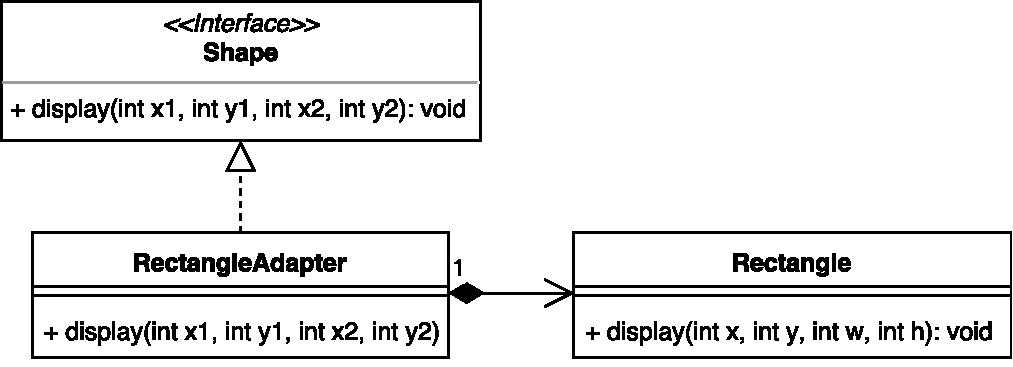
\includegraphics[width=0.8\linewidth]{adapter-ex.pdf}
    \caption{UML diagram over the Adapter example used}
    \label{fig:adapter-uml}
\end{figure}

\subsection{Template method Pattern}
\label{sub:template_method_pattern}
In the Template method pattern one defines a skeleton of an algorithm, but deferring some steps to subclasses.
It solves a similar problem as the Strategy pattern, although Strategy relies on composition rather than inheritance.
The primary use case for the Template method pattern is to reduce duplicated code between two or more classes that have much in common in terms of source code, but differ in some details ~\cite{gamma1993:gof}.

Consider an following example in which there exists several different animal classes: Cat, Sheep, and so on, which all have a unique name and make a unique noise.
Suppose that allthese animals share a \emph{what\_does\_it\_say} method which prints the animals name and the noise they make.
Applying the Template method pattern to this problem results in an abstract class Animal which contains the \emph{what\_does\_it\_say} method but defers the \emph{name} and \emph{noise} methods to subclasses Sheep, Cat, etc.
For simplification, only the Sheep animal will be considered.
See \autoref{fig:template-method-uml} for an UML diagram of the example.

\begin{figure}[htpb]
    \centering
    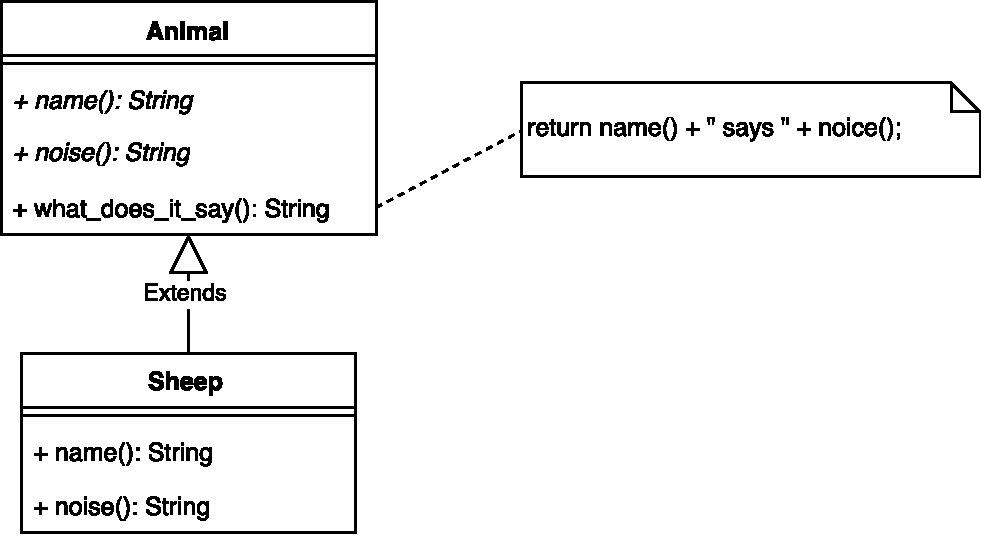
\includegraphics[width=0.8\linewidth]{template-method-ex.pdf}
    \caption{UML diagram over the Template method example used}
    \label{fig:template-method-uml}
\end{figure}

\subsection{Builder Pattern}
\label{sub:builder_pattern}

The Builder design patter primary intent to reuse the same construction process to create multiple different representations by separating the construction of a complex object from its representation.
The main use case for the Builder pattern is to avoid an rapidly expanding set of constructors which can be a result of complex object.
By separating the creation to separate class, a Builder, from the object itself the complexity of the original class is reduced~\cite{gamma1993:gof}.

The example which will be used in this paper is the following.
Suppose there is some threading library in which have a Process class which is rather complex.
Introducing the Builder pattern results in the creation of a Command class which holds intermediate state representing the parameters to be used in the constructor of the Process class.
This state is initialized with some common default values and can then be altered by method calls to a Command instance, and then by calling the \emph{spawn} method an actual instance of the Process object will be created.
For an UML diagram depicting the example, see \autoref{fig:builder-uml}.

\begin{figure}[htpb]
    \centering
    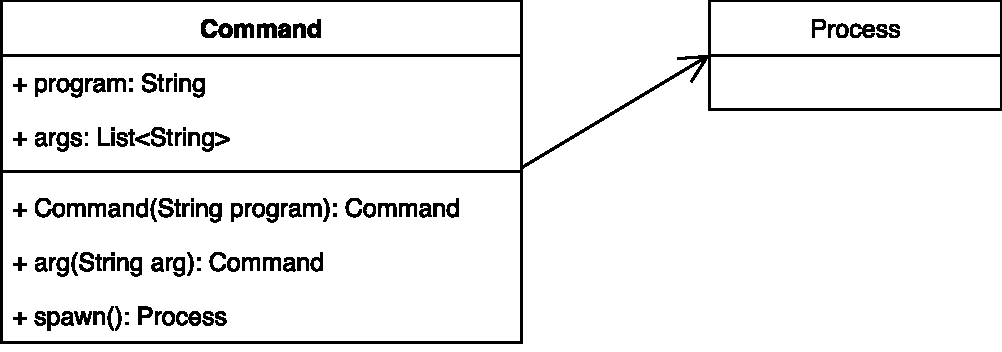
\includegraphics[width=0.8\linewidth]{builder-ex.pdf}
    \caption{UML diagram over the Builder example used}
    \label{fig:builder-uml}
\end{figure}

\subsection{Rust}
\label{sub:rust}
The Rust programming language is a relatively new language, only started in 2006 by Gradon Hoare.
Since then the project has been primarily backed by the Mozilla Foundation~\cite{rustorg2017:faq}.
Rust is a system level programming aimed at performance and critical systems.
It's main feature it boosts is that it guarantees memory safety without any run-time overhead, even over multiple threads~\cite{matsakis:2014:rustlang},~\cite{reed2015:proof}.
Otherwise the language tries to solve problems where languages like C++ currently are most common.

\emph{Traits} is the main way to express abstractions in Rust, and on the surface they are very similar to what would be called an \emph{Interface} in most other languages.
Similar to interfaces they allow the programmer to declare methods with arguments and return values for yet to be implemented types.
Those types when they are later created must implement methods with the given signature to satisfy the interface.
There are however some key differences between traits and typical interfaces in other languages~\cite{rustblog2015:traits}:

\begin{itemize}
    \item
        Traits can not only require methods to be implemented, but can also provide default implementations. This allows Traits to fill a role similar to abstract classes.
        Note that Java added support for this in version 8~\cite{oracle:java_default}.
    \item
        Traits can not only be implemented for new user level types, but also for existing types as the Trait implementation is completely separate from the type declaration.
    \item
        Traits can require constants to be specified as well as methods.
    \item
        Traits can both be statically and dynamically dispatched.
\end{itemize}

\emph{Polymorphism} is the language construct which allows for a single interface to represent multiple different types~\cite{bjarne:polymorphism}.
In Rust polymorphism is achieved using Traits, and it comes both in form of static dispatch and dynamic dispatch.

For static dispatch Rust uses generics which are very similar to the way C++ templates work, i.e the compiler will instantiate multiple versions of the function for each unique type satisfying the generic bounds.
This means that generics results in zero abstraction overhead.
There is also support for dynamic dispatch, i.e dispatch at run-time when indirection is really needed.
For instance when we want to operate on a list of elements of a Trait type but varying concrete types.
Here generics will not work since the concrete types are different.
Furthermore we cannot simply pass a Trait as a value to methods as the compiler generally need to know the exact size of parameter list for functions/methods and the size of a Trait is unknown.
Therefor the types which we want to do dynamic dispatch for must be either ``Boxed``, which is done by wrapping the value in a unsized reference called a \emph{Box}, or passed as a reference~\cite{rustblog2015:traits}.
See \autoref{fig:dispatch-impl} for an example on both static and dynamic dispatch.
\begin{figure}[ht]
    \begin{minted}[autogobble, breaklines=true]{rust}
        trait Animal {
            /// Methods to be implemented
            fn name(&self) -> &'static str;
            fn noise(&self) -> &'static str;
        }

        /// Static dispatch: generic function, compiler will instantiate concrete functions for each caller, e.g. Sheep, Cat etc
        fn what_does_it_say<T: Animal>(animal: &T) {
            println!("{} goes {}", animal.name(), animal.noise());
        }
        /// Dynamic dispatch: Use Box pointer reference
        fn what_does_it_say2(animal: &Box<Animal>) {
            println!("{} goes {}", animal.name(), animal.noise());
        }

    \end{minted}
    \caption{Static and dynamic dispatch in Rust}
    \label{fig:dispatch-impl}
\end{figure}



\section{Results}
The \emph{Adapter} implementation for the example used in \autoref{sub:adapter_pattern} in the Rust programming language can be seen in \autoref{fig:adapter-impl}.
Here the implementation uses the fact that Rust allows for the implementation of Traits for existing types, meaning that we can directly implement the Shape trait onto the Rectangle type.
Where as in Java and similar langauges we have to create wrapper class, \emph{RectangleAdaper}, which implements the Shape interface and also contains a Rectangle instance to which it forwards calls to.
Java implementation therefor follows the given UML diagram presented in \autoref{sub:adapter_pattern} unlike the Rust implementation which forgoes the need for an actual adapter class entirely.
For the Java implementation see \autoref{fig:adapter-java-impl}.
The derived software metrics for the implementations can be seen in \autoref{tab:adapter-metrics}.
We see that the Rust implementation introduced one new interface (Trait) but no new classes unlike Java which both introduced a new interface, and a new class.
Furthermore we see that the Java implementation has a CBO value of 1 where as the Rust implementation has value of 0.
This due to the fact the adapter class introduced in Java needs to forward requests to an instance of the actual Rectangle class.

\begin{table}[hbtp]
    \centering
    \caption{Software metrics for Adapter implementation}
    \label{tab:adapter-metrics}
    \begin{tabular}{lllll}
        & DSCI   & DIT  & CBO   &  \\
        Rust & 2 & 0    & 0     &  \\
        Java & 3 & 0    & 1     &  \\
    \end{tabular}
\end{table}

For the \emph{Template method} implementation in Rust, seen in \autoref{fig:template-impl}, we use Rust's notion of default methods in traits to establish the shared behavior between different concrete Animals.
The other methods, \emph{name} and \emph{noise}, are not given any default implementation and therefor has to be implemented by the concrete types such as \emph{Sheep}.
In Java, see \autoref{fig:template-java-impl} we use a abstract class to represent the Animal trait, letting \emph{name} and \emph{noise} be abstract methods to be implemented, and let \emph{Sheep} be a concrete class inheriting from \emph{Animal}.
The metrics calculated from the implemenations can be seen in \autoref{tab:template-metrics}.
Both in Java and Rust we use two classes/interfaces, only difference being that in Java we utalize class based inheritence resuling in a higher DIT value.

% Should CBO really be 1???
\begin{table}[hbtp]
    \centering
    \caption{Software metrics for Template method implementation}
    \label{tab:template-metrics}
    \begin{tabular}{lllll}
        & DSCI   & DIT  & CBO   &  \\
        Rust & 2 & 0    & 1     &  \\
        Java & 2 & 0.5  & 1     &  \\
    \end{tabular}
\end{table}

In the \emph{Builder} implementation in Rust we have two concrete types: \emph{Command} and \emph{Process}.
Using the \emph{new} method we instantiate a new \emph{Command} and setting the default state needed for creating a \emph{Process} instance.
Then using the different methods we can alter this \emph{Command} state.
Note that all methods except the \emph{Spawn} method return a mutable \emph{Command} reference, allowing us the chain the commands together like $Command::new("ls").arg("l").spawn()$.
In Java we would also have two concrete classes working in a almost identical way, returning $this$ in the different methods would work similarly, allowing us to chain commands together.
From the implementations the metric values seen in \autoref{tab:builder-metrics} is calculated.

\begin{table}[hbtp]
    \centering
    \caption{Software metrics for Builder implementation}
    \label{tab:builder-metrics}
    \begin{tabular}{lllll}
        & DSCI   & DIT  & CBO   &  \\
        Rust & 2 & 0    & 1     &  \\
        Java & 2 & 0    & 1     &  \\
    \end{tabular}
\end{table}

\begin{figure}[btp]
    \begin{minted}[autogobble, breaklines=true]{rust}
        /// Legacy component to be adapted
        pub struct Rectangle;
        impl Rectangle {
            fn display(&self, x: i32, y: i32, w: i32, h: i32) {
                println!("Show rectangle at {},{} with dimensions: {}, {}", x, y, w, h);
            }
        }

        /// User facing interface to be used
        trait Shape {
            fn display(&self, x1: i32, y1: i32, x2: i32, y2: i32);
        }

        /// Append Trait implementation
        impl Shape for Rectangle {
            fn display(&self, x1: i32, y1: i32, x2: i32, y2: i32) {
                Rectangle::display(self, x1, y1, x2-x1, y2-y1);
            }
        }
    \end{minted}
    \caption{Adapter implementation in Rust}
    \label{fig:adapter-impl}
\end{figure}

\begin{figure}[btp]
    \begin{minted}[autogobble, breaklines=true]{rust}
        trait Animal {
            /// Methods deferred to subtypes
            fn name(&self) -> &'static str;
            fn noise(&self) -> &'static str;

            // Trait default implementation, algorithm skeleton
            fn what_does_it_say(&self) {
                println!("{} goes {}", self.name(), self.noise());
            }
        }

        /// "Subtype" Sheep, implements the Animal Trait
        struct Sheep;
        impl Animal for Sheep {
            fn name(&self) -> &'static str {
                "Sheep"
            }

            fn noise(&self) -> &'static str {
                "baaaaah!"
            }
        }
    \end{minted}
    \caption{Template method implementation in Rust}
    \label{fig:template-impl}
\end{figure}

\begin{figure}[btp]
    \begin{minted}[autogobble, breaklines=true]{rust}
        /// Builder to create a Process instance
        pub struct Command {
            program: &str,
            args: Vec<&str>,
        }

        impl Command {
            /// Constructor, set default values
            pub fn new(program: &str) -> Command {
                Command {
                    program: program,
                    args: Vec::new()
                }
            }

            /// Add an argument to pass to the program.
            pub fn arg<'a>(&'a mut self, arg: &str) -> &'a mut Command {
                self.args.push(arg);
                self
            }

            /// Executes the command as a child process, which is returned.
            /// Actually builds the instance
            pub fn spawn(&self) -> IoResult<Process> {
                ...
            }
        }
    \end{minted}
    \caption{Builder implementation in Rust}
    \label{fig:builder-impl}
\end{figure}

\begin{figure}[btp]
    \begin{minted}[autogobble, breaklines=true]{java}
        interface Shape {
            void display(int x1, int y1, int x2, int y2);
        }

        class Rectangle {
            public void draw(int x, int y, int w, int h) {
                System.out.println("Show rectangle at " + x + ", " + y + " with dimensions: " + w + ", " + h); 
            }
        }

        class RectangleAdapter implements Shape {
            private Rectangle adaptee;

            public RectangleAdapter() {
                this.adaptee = new Rectangle();
            }

            @Override
            public void draw(int x1, int y1, int x2, int y2) {
                adaptee.display(x1, y1, x2-x1, y2-y1);
            }
        }
    \end{minted}
    \caption{Adapter implementation in Java}
    \label{fig:adapter-java-impl}
\end{figure}

\begin{figure}[btp]
    \begin{minted}[autogobble, breaklines=true]{java}
        abstract class Animal {
            abstract String name();
            abstract String noise();

            void what_does_it_say() {
                System.out.println(this.name() + " goes " + this.noise());
            }
        }

        // Sheep subclass, extends Animal 
        class Sheep extends Animal {
            public String name() {
                return "Sheep";
            }

            public String noise() {
                return "baaaaah!";
            }
        }
    \end{minted}
    \caption{Template method implementation in Java}
    \label{fig:template-java-impl}
\end{figure}

\begin{figure}[btp]
    \begin{minted}[autogobble, breaklines=true]{java}
        class Command {
            private String program;
            private List<String> args;

            public Command(String program) {
                this.program = program;
                this.args = new ArrayList<String>();
            }

            // Add an argument to pass to the program.
            public Command arg(String arg) {
                this.args.add(arg);
                return this;
            }

            // Executes the command as a child process, which is returned.
            // Actually builds the instance
            public Process spawn() {
                ...
            }

        }
    \end{minted}
    \caption{Builder implementation in Java}
    \label{fig:builder-java-impl}
\end{figure}

\section{Discussion}

% Discuss that the metrics are very similar
% Discuss that the traits have some key advantages and disadvantages 
% Discuss that the metrics may not be that good for measuring non object oriented languages 

From the results above we that the implementions in Rust and Java are quite similar which is also reflected in the metrics. 
There are however some key differences to be noted.

From the Adapter pattern example used we see that Rust's support for implementation of traits for existing types all but eliminates the need for the pattern entirely.
By having trait behavior for a type be seperate from the data of that type we are able to extend the functionallity of existing types without effecting the existing code base.
Suppose we had $N$ number of legacy components which we wanted to implement the Shape trait, then in Java we would have introduced $N$ new Adapter classes. 
In Rust we would have added zero new classes according to the definition given in \autoref{sub:software_metrics}, i.e the size of introducing $N$ adapter patterns would be constant.
This strange result points to a flaw in the definition of a class in Rust as given in this paper.
However there exists only the following options all producing unreasonable results:
\begin{itemize}
    \item The type and all implementations counts as one class
    \item The type and default implementation counts as one class, each trait implementation constitutes an additional class
\end{itemize}
By the second definition we would for the template example we would have three classes: Aniaml, struct Sheep, and the implementation block of Animal for Sheep.
Continuing in the same direction the standard vector collection \emph{vec} in Rust would constitute over a hundred classes~\cite{rustdoc:vec}.
This I believe points to a more general problem of using specifically object oriented metrics for evaluating languges which are not traditionally object oriented.
Two possible solutions would be either to use non object oriented metrics such as number of lines of code (LOC) with the downside of not being able to reason about higher level constructs and for instance coupling easily, or to only use object oriented metrics for which no interpretations would have to be made which could greatly reduce the number of availble metrics when comparing certain languages.

In fact, the implementations of traits are scope bound mening that we can even define behavior local to a particual module.
By allowing adding behavior in this way we also remove the need converting between adapters and adaptees in the source code mediating source code between the client which wishes the use the adapter and the rest of the code base which may use the legacy componen.
Unlike in Java where we would practically need to introduce a facade between the existing code base and the client which translates input of legacy instances into adaptered instances and output of adaptered instances into legacy instances.
This in turn has a great effect of the maintainability of the source code, since the cost of reusing existig components is minimized.

Regaring the template method implementations we see strikingly similar solutions.
Traits with default implementations fills a role similar to that of a abstract class in Java and many other languges.
However, let there be known that it is not equivalent to an abstract class since a Rust trait cannot hold any state.
Therefor it becomes difficult to replicate the behavior of a more complex case of the template method, specifically when the algorithm skeleton and surronding methods rely on state between method calls.
In this case in Rust's one should probably look to the similar Strategy pattern instead, since it does not require any class based inheritence.
Furthermore one should proabably prefer Streatgy generally over template method any way since it works based on composition rather than inheritence~\cite[p.32]{gamma1993:gof}.

Finally, the Builder pattern is practically identical between the two langauges, disregarding syntax differences.
Becuase Rust does not support function/method overloading the Builder pattern becomes very useful.
In fact, It is so useful that it is used multiple times in the Rust standard library and the example used in this paper is a simplification of the actual \emph{Command} builder in the Rust standard library~\cite{rustdoc:command}.
There even exists Rust libraries that are able to automatically derive, i.e let the compiler generate source code, builder patterns for arbirary types~\cite{cratesio:builder}.
Not having support for multiple constructors means that a programmer in Rust would have to create and maintain a large number of uniquely names methods that consitute different constructors, leading to poor maintainability.
Where as with a Builder there is a separation of the construction and the behavior of a type thus resolving the programmer for creating variants of the "new" method and instead only adding methods when new paramters to the actual constructor is added.

It is important to note however that overloading can in some sense be achive through trait implementations since we can over different trait implementations name our methods identically, even with the same parameter list.
Using traits does of course imply that those traits need to be created also, so there is not a full overlap.
However creating objects in different contexts may also imply that they are used in different contexts, and therefor multiple traits may be a good idea to better hold to the idea of the dependency inversion principle.

Finally, observing the metric results above we see that the DIT values are all zeroed for the Rust implementations.
Becuase Rust has no equivalent notion of class based inheritance we can see that 

\section{Conclusion}
TODO: The conclusion goes here.

% trigger a \newpage just before the given reference
% number - used to balance the columns on the last page
% adjust value as needed - may need to be readjusted if
% the document is modified later
%\IEEEtriggeratref{8}
% The "triggered" command can be changed if desired:
%\IEEEtriggercmd{\enlargethispage{-5in}}

% references section

% can use a bibliography generated by BibTeX as a .bbl file
% BibTeX documentation can be easily obtained at:
% http://mirror.ctan.org/biblio/bibtex/contrib/doc/
% The IEEEtran BibTeX style support page is at:
% http://www.michaelshell.org/tex/ieeetran/bibtex/
%\bibliographystyle{IEEEtran}
% argument is your BibTeX string definitions and bibliography database(s)
%\bibliography{IEEEabrv,../bib/paper}
%
% <OR> manually copy in the resultant .bbl file
% set second argument of \begin to the number of references
% (used to reserve space for the reference number labels box)
%\begin{thebibliography}{1}
%
%\bibliographystyle{./IEEEtran}

\clearpage
\bibliographystyle{IEEEtranN}
\bibliography{IEEEabrv,references}




% that's all folks
\end{document}
